\documentclass[a4paper,12pt]{report}

% pakiety dla j�zyka polskiego
\usepackage{polski}
\usepackage[cp1250]{inputenc}

% pakiet odpowiedzialny za linki
\usepackage[colorlinks=true,urlcolor=blue,linkcolor=red,citecolor=green]{hyperref}

%\pagestyle{plain}
%\usepackage[pdftex]{color,graphics}
\usepackage{graphicx}
\usepackage{fancyhdr}

%1,5 linii odst�pu
\linespread{1.3}

% ********************* pocz�tek dokumentu ***********************
\begin{document}

%	\pagestyle{fancy}
	\cfoot{\thepage}

% ********************* Tworzy spis tre�ci ***********************
	\tableofcontents
	\newpage

% ****************************************************************
% Wst�p
\section{Wst�p} \label{roz:wstep}
	Wraz ze wzrostem zapotrzebowania na pozyskanie nowych klient�w, a tym samym kontrakt�w oraz z naciskami ze strony organizacji ochrony �rodowiska, aby zredukowa� liczb� drukowanych dokument�w, coraz wi�cej firm decyduje si� na generowanie i wymian� dokument�w mi�dzy pracownikami (i/lub swoimi oddzia�ami) w formie elektronicznej. Je�li wymiana tych dokument�w dokonywana jest w w�skim gronie pracownik�w, mo�emy by� w 100\% pewni, �e dokument jest autentyczny i w formie niezmienionej. Problem zaczyna si�, gdy musimy wymienia� dokumenty z naszymi pracownikami lub partnerami handlowymi w r�nych miastach lub nawet krajach. Wtedy nie mo�emy mie� pewno�ci, �e dokument wys�any jest tym samym dokumentem, kt�ry otrzymali�my. Przy dzisiejszej technologii dokument taki m�g� zosta� przechwycony przez osoby niepowo�ane (trzecie) i/lub zmieniony w celu zmylenia adresata lub korzy�ci maj�tkowych.

Rozwi�zaniem problemu stwierdzenia autentyczno�ci dokumentu oraz pewno�ci, �e nadawca jest tym, za kogo si� podaje, jest podpis elektroniczny (cyfrowy). Narz�dziem, kt�re nam to w prosty spos�b umo�liwia jest j�zyk XML, a dok�adniej \textit{XML Signature}.

	\newpage

% Cel pracy
\section{Cel pracy} \label{roz:cel_pracy}
	Praca ma na celu zaprezentowanie mo�liwo�ci, jakie daje kryptografia oraz j�zyk XML w zakresie podpisu elektronicznego.

\textit{ZA MA�O!}

% Struktura pracy
\section{Struktura pracy} \label{roz:struktura_pracy}
	\ref{roz:wstep} - ten rozdzia�, ...

Dalsza cz�� struktury pracy powstanie po napisaniu pracy.

% Rozdzia� 1
\chapter{Pocz�tek...} \label{roz:rozdzial_1}
	Na pocz�tku by�o pismo wykszta�cone niezale�nie w wielu kulturach stanowi�o niezbadan� tajemnic� dla tych, kt�rzy nie potrafili czyta�. Szybko jednak zrodzi�a si� konieczno�� ukrycia informacji r�wnie� przed tymi, kt�rym umiej�tno�� ta nie by�a obca. Najbardziej oczywistym rozwi�zaniem by�o schowanie tajnej wiadomo�ci przed lud�mi, kt�rzy mogliby j� odczyta�. Takie zabiegi wkr�tce jednak przesta�y wystarcza�. Wiadomo�� mog�a zosta� odnaleziona podczas wnikliwego przeszukania, a wtedy tajne informacje dosta�yby si� w r�ce wroga. A gdyby uda�o si� napisa� list dzia�aj�cy na zasadzie �drugiego dna"? Z pozoru zawiera�by on b�ahe tre�ci, jednak je�li adresat wiedzia�by, gdzie i jak szuka�, m�g�by dotrze� do �mniej niewinnych" informacji. Tak narodzi�a si� steganografia.

\section{Steganografia}
\textit{Steganografia} to og� metod ukrywania tajnych przekaz�w w wiadomo�ciach, kt�re nie s� tajne. Jej nazwa wywodzi si� od greckich s��w: \textit{steganos} (ukryty) oraz \textit{graphein} (pisa�). W przesz�o�ci stosowano wiele wymy�lnych sposob�w osi�gni�cia tego efektu. Popularny niewidzialny atrament to jeden z najbardziej znanych przyk�ad�w steganografii. Pierwsze zapiski na temat stosowania tej sztuki znale�� mo�na ju� w ksi�gach z V wieku p.n.e. Przyk�adem mo�e by� opisana przez Herodota historia Demaratosa, Greka, kt�ry ostrzeg� Spartan przed przygotowywan� przeciw nim ofensyw� wojsk perskich. Nie m�g� on wys�a� oficjalnej wiadomo�ci do kr�la, zeskroba� wi�c wosk z tabliczki i wyry� tekst w drewnie. Nast�pnie ponownie pokry� tabliczk� woskiem i wr�czy� pos�a�cowi. Czysta tabliczka nie wzbudzi�a podejrze� perskich patroli i bezpiecznie dotar�a do celu. Tam, co prawda, d�ugo g�owiono si� nad jej znaczeniem, wkr�tce jednak �ona sparta�skiego wodza Leonidasa wpad�a na pomys� zeskrobania wosku, co pozwoli�o odkry� tajn� wiadomo��.

W miar� post�pu technicznego, a tak�e rozwoju samej steganografii, powstawa�y coraz wymy�lniejsze metody ukrywania wiadomo�ci. Znana jest na przyk�ad metoda ukrywania wiadomo�ci w formie kropki w tek�cie drukowanym, stosowana podczas II wojny �wiatowej. Wiadomo�� by�a fotografowana, a klisza pomniejszana do rozmiar�w oko�o $mm^2$ i naklejana zamiast kropki na ko�cu jednego ze zda� w li�cie. Obecnie bardzo popularne jest ukrywanie wiadomo�ci w plikach graficznych. Kolejne przyk�ady mo�na mno�y�, jednak nawet najbardziej wymy�lne z nich nie gwarantuj�, i� wiadomo�� nie zostanie odkryta. Konieczno�ci� sta�o si� zatem wynalezienie takiego sposobu jej zapisywania, kt�ry gwarantowa�by tajno�� nawet w przypadku przechwycenia przez osoby trzecie.

\section{Kryptografia}
Nazwa \textit{kryptografia} r�wnie� wywodzi si� z j�zyka greckiego (od wyraz�w \textit{kryptos} � ukryty i \textit{graphein} � pisa�). Jej celem jest utajnienie znaczenia wiadomo�ci, a nie samego faktu jej istnienia. Podobnie jak w przypadku steganografii, data jej powstania jest trudna do okre�lenia. Najstarsze znane przyk�ady przekszta�cenia pisma w form� trudniejsz� do odczytania pochodz� ze staro�ytnego Egiptu, z okresu oko�o 1900 roku p.n.e. Pierwsze tego typu zapisy nie s�u�y�y jednak ukrywaniu tre�ci przed osobami postronnymi, a jedynie nadaniu napisom formy bardziej ozdobnej lub zagadkowej. Skrybowie zapisuj�cy na �cianach grobowc�w historie swych zmar�ych pan�w �wiadomie zmieniali niekt�re hieroglify, nadaj�c napisom bardziej wznios�� form�. Cz�sto celowo zacierali ich sens, zach�caj�c czytaj�cego do rozwi�zania zagadki. Ten element tajemnicy by� wa�ny z punktu widzenia religii. Sk�ania� on ludzi do odczytywania epitafium i tym samym do przekazania b�ogos�awie�stwa zmar�emu. Nie by�a to kryptografia w �cis�ym tego s�owa znaczeniu, zawiera�a jednak dwa podstawowe dla tej nauki elementy � przekszta�cenie tekstu oraz tajemnic�.

Na przestrzeni kolejnych 3000 lat rozw�j kryptografii by� powolny i dosy� nier�wny. Powstawa�a ona niezale�nie w wielu kr�gach kulturowych, przybieraj�c r�ne formy i stopnie zaawansowania. Zapiski na temat stosowania szyfr�w znaleziono na pochodz�cych z Mezopotamii tabliczkach z pismem klinowym. Ich powstanie datuje si� na 1500 rok p.n.e. W II w. p.n.e. grecki historyk Polibiusz opracowa� system szyfrowania oparty na tablicy przyporz�dkowuj�cej ka�dej literze par� cyfr (tabela~\ref{tab:TablicaPolibiusza}).
\begin{table}
	\centering
		\begin{tabular}{|c|c|c|c|c|c|}
			\hline
			  & 1 & 2 & 3 & 4 & 5 \\ \hline
			1 & A & B & C & D & E \\ \hline
			2 & F & G & H & I/J & K \\ \hline
			3 & L & M & N & O & P \\ \hline
			4 & Q & R & S & T & U \\ \hline
			5 & V & W & X & Y & Z \\ \hline
		\end{tabular}
	\caption{Tablica Polibiusza}
	\label{tab:TablicaPolibiusza}
\end{table}
W p�niejszych czasach tablica ta sta�a si� podstaw� wielu system�w szyfrowania. Przekszta�cenie liter w liczby dawa�o mo�liwo�� wykonywania dalszych przekszta�ce� za pomoc� prostych oblicze� lub funkcji matematycznych. Metod� Polibiusza uzupe�nion� kilkoma dodatkowymi utrudnieniami kryptoanalitycznymi zastosowa�a mi�dzy innymi niemiecka armia przy opracowywaniu wspomnianego na wst�pie systemu szyfruj�cego ADFGX oraz jego udoskonalonej wersji ADFGVX.

Pierwsze wzmianki dotycz�ce stosowania kryptografii w celach politycznych pochodz� z V w. p.n.e. z Indii. Wymieniana jest ona jako jeden ze sposob�w zdobywania informacji przez przebywaj�cych za granic� ambasador�w. Sekretne pismo wspomniane jest r�wnie� w s�ynnej Kamasutrze � figuruje tam jako jedna z 64 sztuk, kt�re kobieta powinna zna�.

Og�lnie stosowane w staro�ytno�ci metody kryptografii mo�na podzieli� na dwa rodzaje � przestawianie i podstawianie. W pierwszym przypadku nast�powa�a zamiana szyku liter w zdaniach, czyli, innymi s�owy, tworzony by� anagram. Przyk�adem szyfrowania przestawieniowego jest pierwsze znane urz�dzenie szyfruj�ce � \textit{sparta�ska scytale} z V w. p.n.e. Mia�a ona kszta�t pr�ta o podstawie wielok�ta, na kt�ry nadawca nawija� sk�rzany pas. Wiadomo�� pisana by�a wzd�u� pr�ta, po czym odwijano pas, na kt�rym wida� by�o tylko pozornie bezsensown� sekwencj� liter. Potem goniec przenosi� list do adresata, stosuj�c czasem steganograficzne sztuczki, na przyk�ad opasuj�c si� nim i ukrywaj�c tekst po wewn�trznej stronie. Odczytanie wiadomo�ci by�o mo�liwe przy u�yciu scytale o takiej samej grubo�ci, jak� mia� pr�t nadawcy.

Druga, bardziej popularna metoda polega�a na podstawianiu za litery tekstu jawnego innych liter b�d� symboli. Za przyk�ad mo�e tu pos�u�y� szyfr Cezara, najs�ynniejszy algorytm szyfruj�cy czas�w staro�ytnych (jego tw�rc� by� Juliusz Cezar). Szyfr ten opiera� si� na zast�pieniu ka�dej litery inn�, po�o�on� o trzy miejsca dalej w alfabecie. W ten spos�b na przyk�ad wiadomo�� o tre�ci Cesar przekszta�ca si� w Fhvdu. Adresat znaj�cy spos�b szyfrowania w celu odczytania wiadomo�ci zast�powa� ka�d� liter� tekstu tajnego liter� po�o�on� o trzy miejsca wcze�niej w alfabecie.

% Szyfr Cezara - rysunek do wstawienia

Szyfry przyporz�dkowuj�ce ka�dej literze alfabetu jawnego dok�adnie jedn� liter�, kombinacj� cyfr lub symbol nazywamy szyframi monoalfabetycznymi. W przypadku szyfru Cezara uk�ad alfabetu tajnego zawsze pozostawa� ten sam. Znacznie bezpieczniejszym rozwi�zaniem by�o dokonywanie w nim okresowych zmian tak, aby znajomo�� metody szyfrowania nie wystarcza�a do odczytania wiadomo�ci.

Stanowi�o to jednak utrudnienie r�wnie� dla adresata. Musia� on dodatkowo posiada� klucz (uk�ad liter lub symboli w alfabecie tajnym). Tak powsta� najwi�kszy problem w historii kryptografii � dystrybucja klucza. Raz przechwycony klucz stawa� si� bezu�yteczny, gdy� wiadomo�ci szyfrowane za jego pomoc� nie by�y ju� bezpieczne. O ile w przypadku wymiany wiadomo�ci mi�dzy dwiema osobami nie by�a to z regu�y du�a przeszkoda (wystarczy�o ustali� nowy klucz), o tyle w przypadku szyfrowania na potrzeby wojskowe rodzi�o to bardzo wiele problem�w. Trzeba by�o dostarczy� nowy klucz do wszystkich jednostek i to mo�liwie szybko, gdy� ka�da przechwycona przez wroga wiadomo�� stawa�a si� dla niego �atwa do odczytania.

Istniej� dwie podstawowe grupy algorytm�w szyfrowania.

% ----------------------------------------------------------------------------

\section{Szyfry z kluczem symertycznym} \label{roz:szyfr_sym}
Przy szyfrowaniu wiadomo�ci kluczem symertycznym, klucz u�ywany do jej zaszyfrowania jest identyczny z kluczem wymaganym do ich odszyfrowania (rys. \ref{rys:klucz_symetryczny}). Oznacza to, �e najpierw nadawca i odbiorca musz� wsp�lnie okre�li� klucz, jakiego b�d� u�ywa� do szyfrowania korespondencji mi�dzy sob�. Oznacza to, �e przy korespondencji z np. 10 kontrahentami musimy posiada� 10 r�nych kluczy, co mo�e stanowi� problem z okre�leniem, kt�ry klucz powinni�my u�y�. Globalnie oznacza to, �e dla np. 10 os�b trzeba wygenerowa� a� 45 r�nych kluczy, ale przy np. 100 osobach ju� trzeba wygenerowa� 4950 r�nych kluczy.

%rysunek - klucz symetryczny
\begin{figure}
	\begin{center}
		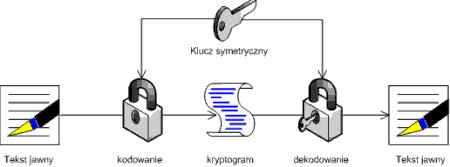
\includegraphics{kryptografia//rysunki//klucz_sym.jpg}
		\caption{Schemat szyfrowania kluczem symetrycznym. �r�d�o \cite{vpn_svera}} \label{rys:klucz_symetryczny}
	\end{center}
\end{figure}

% ----------------------------------------------------------------------------

\section{Szyfry z kluczem asymertycznym} \label{roz:szyfr_asym}
W algorytmach szyfrowania asymetrycznego klucze szyfrowania i deszyfracji s� r�ne i s� w posiadaniu r�nych os�b (rys. \ref{rys:klucz_asymetryczny}). Oznacza to, �e ka�da osoba chc�ca szyfrowa� wiadomo�ci musi posiada� dwa klucze, \textbf{publiczny} i \textbf{prywatny}. Jak sama nazwa wskazuje klucz publiczny jest udost�pniany wszystkim zainteresowanym, natomiast klucz prywatny musi pozosta� tany. Zalet� szyfrowania asymetrycznego jest to, �e ka�da osoba musi posiada� jeden klucz prywatny (sw�j) oraz klucze publiczne os�b, z kt�rymi chce korespondowa�. Oznacza to, �e musimy posiada� mniejsz� ilo�� kluczy ni� w przypadku szyfrowania kluczem symetrycznym. Globalnie oznacza to, �e dla np. 10 os�b trzeba wygenerowa� tylko 20 kluczy, a dla np. 100 os�b tych kluczy potrzeba wygenerowa� tylko 200. Jak wida� r�nica w liczbie generowanych kluczy jest kolosalna, dlatego obecnie na �wiecie spos�b ten jest najcz�ciej stosowany.

%rysunek - klucz asymetryczny
\begin{figure}
	\begin{center}
		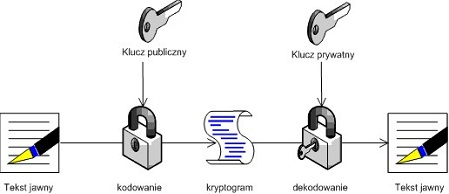
\includegraphics{kryptografia//rysunki//klucz_asym.jpg}
		\caption{Schemat szyfrowania kluczem asymetrycznym. �r�d�o \cite{vpn_svera}} \label{rys:klucz_asymetryczny}
	\end{center}
\end{figure}

% ----------------------------------------------------------------------------

\section{Podpis cyfrowy}
\textbf{Podpis cyfrowy} jest to matematyczny spos�b potwierdzania autentyczno�ci cyfrowego dokumentu. Istnieje wiele schemat�w podpis�w cyfrowych, obecnie jednak najpopularniejszym jest schemat podpisu dokument�w cyfrowych w~systemach kryptograficznych z kluczem publicznym i jednokierunkow� funkcj� skr�tu - w systemie tym do oryginalnej wiadomo�ci do��czany jest skr�t dokumentu, zaszyfrowany prywatnym kluczem nadawcy. Potwierdzenie autentyczno�ci wiadomo�ci jest mo�liwe po odszyfrowaniu skr�tu kluczem publicznym nadawcy i por�wnaniu go z wytworzonym skr�tem odebranego dokumentu \cite{wiki_podpis_cyfrowy}.

Podpisywanie si� pod dokumentami jest nieod��czn� cz�ci� handlu. Wraz z rozwojem handlu elektronicznego narodzi�a si� potrzeba opracowania elektronicznych odpowiednik�w podpis�w. Protoko�y podpisu elektronicznego s� pr�b� rozwi�zania tego problemu. W Polsce prace nad wprowadzeniem podpisu elektronicznego ruszy�y na pocz�tku roku 2001. Odpowiednia ustawa zosta�a uchwalona 18 wrze�nia tego samego roku. Kolejny rok zaj�o wprowadzanie odpowiednich akt�w wykonawczych, w wyniku czego oficjalnie w polskim prawie podpis elektroniczny funkcjonuje dopiero od 16 sierpnia 2002. Powsta�o kilka Centr�w Certyfikacji pozwalaj�cych na wyrobienie certyfikatu niezb�dnego do wykonywania podpis�w elektronicznych.

Podobnie jak w przypadku pozosta�ych protoko��w, najpierw trzeba si� zastanowi�, jakie warunki musi spe�nia� poprawnie wykonany podpis elektroniczny. Dopiero wtedy mo�na zacz�� my�le� nad zastosowaniem konkretnych mechanizm�w kryptograficznych.
Z pewno�ci� podpis powinien jednoznacznie wskazywa� na to�samo�� podpisuj�cego. Ponadto powinien by� niepodrabialny. Osoba podpisuj�ca nie mo�e p�niej wyprze� si� z�o�onego podpisu, jak r�wnie� zmieni� tre�ci podpisanego dokumentu. Wreszcie sam podpis nie mo�e zosta� u�yty po raz drugi, ani te� przeniesiony na inny dokument.

W protoko�ach podpisu cyfrowego powy�sze zadania s� realizowane przy u�yciu kryptografii asymetrycznej oraz jednokierunkowych funkcji skr�tu. S� to funkcje jednokierunkowe, generuj�ce jako wynik skr�t o okre�lonej d�ugo�ci. Innymi s�owy dla dowolnie d�ugiej wiadomo�ci (nieprzekraczaj�cej limitu wyznaczonego dla danego algorytmu) wynik b�dzie mia� zawsze ten sam rozmiar (na przyk�ad 160 bit�w). Jest to bardzo przydatna w�a�ciwo��, poniewa� cz�sto podpisywane dokumenty maj� do�� spore rozmiary. Bez funkcji skr�tu obliczenia konieczne do wykonania podpisu znacznie by si� wyd�u�a�y. Podpisywanie skr�tu wiadomo�ci trwa natomiast o wiele kr�cej.

Wygenerowany skr�t wiadomo�ci podpisywany jest z wykorzystaniem klucza prywatnego u�ytkownika. Umo�liwia to ka�demu, kto ma dost�p do odpowiedniego klucza publicznego, zweryfikowanie to�samo�ci podpisuj�cego. Zmiana tre�ci dokumentu uniemo�liwi weryfikacj� podpisuj�cego, a samego podpisu nie mo�na przenie�� na inny dokument.

Opisana procedura to �klasyczny" protok� podpisu cyfrowego. W zale�no�ci od potrzeb tworzone s� r�wnie� inne rozwi�zania. Poni�ej Autor podaje niekt�re z nich.

\subsection{Niezaprzeczalne podpisy cyfrowe}
Nazwa tego typu protoko��w mo�e by� nieco myl�ca, poniewa� protoko�y niezaprzeczalne (opr�cz tradycyjnej funkcji podpisywania dokument�w) uniemo�liwiaj� weryfikacj� podpisu bez zgody podpisuj�cego. Wi��e si� ona jednak z tym, i� podpisuj�cy nie mo�e si� r�wnie� wyprze� swojego podpisu. Protok� tego typu przebiega w nast�puj�cy spos�b:
\begin{itemize}
	\item U�ytkownik A przedstawia u�ytkownikowi B dokument wraz z wykonanym przez siebie podpisem.
	\item U�ytkownik B generuje liczb� losow� i przesy�a j� do u�ytkownika A.
	\item U�ytkownik A dokonuje przekszta�cenia otrzymanej liczby w oparciu o sw�j klucz prywatny. Przekszta�cenie to jest dosy� zawi�e matematycznie, najwa�niejszy jednak jest fakt, i� uzyskanie poprawnego (pasuj�cego do podpisu) wyniku jest mo�liwe tylko przy wykorzystaniu klucza prywatnego osoby podpisuj�cej.
	\item U�ytkownik A wysy�a wynik oblicze� do u�ytkownika B.
	\item Nast�puje weryfikacja podpisu.
\end{itemize}
Mimo wra�liwo�ci na ataki typu Man in the Middle protoko�y tego typu znajduj� liczne zastosowania ze wzgl�du na mo�liwo�� kontrolowania procesu weryfikacji przez osob� podpisuj�c� dokument. Dodatkowe podprotoko�y pozwalaj� na dowodzenie autentyczno�ci podpis�w lub uniemo�liwiaj� wypieranie si� ich.

Przyk�adowe algorytmy realizuj�ce protok� podpisu niezaprzeczalnego to:
\begin{itemize}
	\item \textit{Algorytm Chauma} � oparty na pot�gowaniu modulo liczba pierwsza p,
	\item \textit{Algorytm Boyar-Damagarda} � oparty na algorytmie podpisu cyfrowego EIGamala,
	\item \textit{Algorytm Harna-Yanga} � dla niezaprzeczalnych podpis�w grupowych.
\end{itemize}

\subsection{Niepodrabialne podpisy cyfrowe}
Najpierw wypada si� zastanowi�, jakie cechy musia�by posiada� podpis niepodrabialny. Poniewa� technologia podpisu opiera si� na wykorzystaniu par kluczy publiczny-prywatny, ewentualne fa�szerstwo wymaga�oby znalezienia (lub odtworzenia) odpowiedniego klucza prywatnego. Taka operacja wymaga ogromnej mocy obliczeniowej por�wnywalnej ze z�amaniem szyfru asymetrycznego. Niemniej jednak nie mo�na wykluczy� tego typu atak�w. Jak im przeciwdzia�a�? Ot� jest to niemo�liwe. Fa�szerstwu nie da si� zapobiec, mo�na je jednak wykry�. S�u�� temu protoko�y podpis�w niepodrabialnych. Dla ka�dego klucza publicznego istnieje wiele pasuj�cych kluczy prywatnych. Aby dokona� fa�szerstwa, atakuj�cy musia�by znale�� ten w�a�ciwy, b�d�cy w posiadaniu osoby wykonuj�cej podpis. Tymczasem o wiele wi�ksze jest prawdopodobie�stwo uzyskania innego klucza prywatnego pasuj�cego do badanych podpis�w i klucza publicznego. Podpisy wykonane tym kluczem faktycznie b�d� weryfikowane jako nale��ce do osoby, kt�rej podpis jest podrabiany. Niemniej jednak, je�li zajdzie taka konieczno��, �atwo b�dzie udowodni�, �e dosz�o do fa�szerstwa, poniewa� wykonano je przy u�yciu innego klucza prywatnego. Podpisy s� w takim przypadku odmienne, chocia� pasuj� do tego samego klucza publicznego.

W ten spos�b zniwelowane zostaje ryzyko skutecznego ataku ze strony przeciwnika dysponuj�cego du�� moc� obliczeniow�, nadal jednak istnieje mo�liwo�� podrobienia podpisu poprzez kradzie� w�a�ciwego klucza prywatnego.

\subsection{Podpisy �lepe}
�lepe podpisy cyfrowe opracowano z my�l� o sytuacjach, w kt�rych podpisuj�cy nie powinien pozna� tre�ci podpisywanego dokumentu. By� mo�e wydaje si� to niedorzeczne, a jednak w pewnych okoliczno�ciach mo�e okaza� si� przydatne.

Wyobra�my sobie sytuacj�, w kt�rej jeden z uczestnik�w protoko�u wyst�puje w charakterze notariusza. Potwierdza swoim podpisem dostarczenie pewnego dokumentu przez innego u�ytkownika. Jednocze�nie dostarczyciel chcia�by mie� pewno��, i� notariusz nie pozna informacji zawartych we wspomnianym dokumencie.

Najprostszym rozwi�zaniem w takiej sytuacji jest wykorzystanie tzw. czynnika zaciemniaj�cego. Jest to wybrana losowo zmienna, przez kt�r� u�ytkownik A mno�y wysy�ane do podpisu dane. U�ytkownik B (notariusz) sk�ada podpis pod tak przekszta�conym dokumentem, nie maj�c mo�liwo�ci uzyskania �adnych informacji co do jego tre�ci (o ile zmienna wybrana by�a w spos�b naprawd� losowy), a nast�pnie odsy�a go u�ytkownikowi A. Ten usuwa zaciemnienie i otrzymuje pierwotny dokument wraz z podpisem. Takie rozwi�zanie ma jednak pewn� wad�. U�ytkownik B nie ma �adnej mo�liwo�ci sprawdzenia, czy tak naprawd� nie podpisuje zobowi�zania wp�aty sporej sumy na konto u�ytkownika A. Aby temu zapobiec, udoskonalono ca�� procedur� w poni�ej opisany spos�b. U�ytkownik A przygotowuje dokument do podpisu, po czym wykonuje n jego kopii. Wszystkie kopie, ka�da po przemno�eniu przez inny czynnik zaciemniaj�cy, przesy�ane s� do u�ytkownika B. Ten prosi u�ytkownika A o dostarczenie czynnik�w zaciemniaj�cych dla $n$-1 dokument�w. Wszystkie te dokumenty sprawdzane s� pod k�tem potencjalnego oszustwa. Je�li oka�� si� formalnie poprawne, podpis jest sk�adany pod jedynym nieodszyfrowanym plikiem. Aby m�c oszuka� tak skonstruowany protok�, u�ytkownik A musia�by przewidzie� (a raczej zgadn��), o kt�re czynniki zaciemniaj�ce poprosi go u�ytkownik B. Prawdopodobie�stwo takiego wydarzenia wynosi l/$n$. Innymi s�owy im wi�ksze $n$, tym wi�ksze prawdopodobie�stwo wykrycia z�ych zamiar�w ze strony wysy�aj�cego dokument. Je�li dodamy do tego surow� kar� za wszelkie pr�by oszustwa, protok� powinien zapewni� du�e bezpiecze�stwo.

\subsection{Inne warianty podpisu cyfrowego}
Opr�cz powy�szych wymieni� mo�na r�wnie� inne protoko�y dokonywania podpis�w cyfrowych, opieraj�ce si� na podobnych rozwi�zaniach:
\begin{itemize}
	\item \textit{Podpisy po�rednie} (ang. \textbf{proxy signatures}) pozwalaj� na wstawianie podpis�w przez u�ytkownika B w imieniu u�ytkownika bez znajomo�ci jego klucza prywatnego,
	\item \textit{Podpisy z wyznaczonym potwierdzaj�cym} (ang. \textbf{designated confirmer signatures}) umo�liwiaj� weryfikacj� podpisu przez osob� trzeci�. Dzi�ki temu potwierdzenie poprawno�ci podpisu jest mo�liwe nawet w sytuacji, kiedy osoba podpisuj�ca jest niedost�pna (na przyk�ad ze wzgl�du na chorob� lub wyjazd), a tak�e w przypadku utraty przez ni� klucza prywatnego
	\item \textit{Podpisy grupowe} (ang. \textbf{group signatures}) s�u�� nie tyle sprawdzeniu to�samo�ci podpisuj�cego, ile jego przynale�no�ci do danej grupy. Innymi s�owy protok� obs�uguje przyznawanie uprawnie� w obr�bie okre�lonego zbioru u�ytkownik�w. Podpisy sprawdzane s� jedynie pod k�tem przynale�no�ci danego u�ytkownika do wspomnianego zbioru. Jego to�samo�� mo�e by� jednak ujawniona, je�li zachodz� w�tpliwo�ci co do autentyczno�ci podpisu.
\end{itemize}

	
% Rozdzia� 2
\chapter{Infrastruktura klucza publicznego} \label{roz:pki}
	Skr�t PKI oznacza \textit{infrastruktur� klucza publicznego} (ang. \textbf{Public Key Infrastructure}) i odnosi si� do rozwi�za� maj�cych na celu zarz�dzanie kluczami publicznymi u�ytkownik�w. O ile bowiem wymiana zaszyfrowanej korespondencji mi�dzy znajomymi nie wymaga specjalnego systemu zarz�dzania kluczami szyfruj�cymi, o tyle w przypadku rozwi�za� na wi�ksz� skal� system taki jest konieczny. Mamy w�wczas do czynienia z wi�ksz� liczb� u�ytkownik�w i konieczne jest rozwi�zanie problemu bezpiecznej dystrybucji kluczy. Jak� mamy bowiem gwarancj�, �e pobrany przez nas z serwera klucz publiczny faktycznie nale�y do danej osoby? Mo�e mamy do czynienia z atakiem Man in the Middle? Konieczne staje si� zatem utworzenie zaufanej instytucji, kt�ra potwierdza�aby przynale�no�� kluczy do poszczeg�lnych os�b i organizacji. Tu pojawia si� PKI.

\section{PKI w teorii...}
PKI jest rozwi�zaniem pozwalaj�cym na przypisywanie u�ytkownikom kluczy i uniemo�liwianie fa�szerstw opartych na ich podmienianiu. Jak jednak mia�oby to dzia�a�? Na pocz�tek Autor przedstawia model teoretyczny.

PKI zak�ada istnienie centralnej instytucji obdarzonej powszechnym zaufaniem, kt�rej zadaniem by�oby wydawanie, przechowywanie i udost�pnianie kluczy publicznych oraz udzielanie informacji o nich. Instytucj� tak� nazywamy centrum certyfikacji (stosuje si� r�wnie� skr�t CA pochodz�cy od angielskiej nazwy \textbf{certification authority}). Ka�dy nades�any klucz publiczny podlega procesowi certyfikacji � u�ytkownik, kt�ry go nades�a�, proszony jest o podanie swoich danych osobowych, a te s� przez centrum weryfikowane. Je�li podane informacje oka�� si� prawdziwe, do klucza zostaje przypisany odpowiedni certyfikat, w kt�rym potwierdza si�, i� klucz ten nale�y do danego u�ytkownika. Certyfikat zawiera podpis elektroniczny centrum certyfikacji, dzi�ki czemu ka�dy mo�e zweryfikowa� jego autentyczno��. Jedynym warunkiem jest tutaj og�lna dost�pno�� klucza publicznego danego centrum.
Klucze u�ytkownik�w s� przechowywane w centrum certyfikacji i powszechnie udost�pniane. W ka�dej chwili mo�liwe jest usuni�cie w�asnego klucza z bazy danych (na przyk�ad w przypadku kompromitacji klucza prywatnego).

Przedstawione rozwi�zanie wygl�da elegancko i sprawia wra�enie bezpiecznego. Mamy oto zaufan� instytucj� umo�liwiaj�c� wszystkim bezpieczn� komunikacj� z u�yciem kryptografii asymetrycznej. Rzeczywisto��, jak zwykle, wygl�da nieco inaczej.

\section{...i w praktyce}
Opisany powy�ej model PKI nie ma prawa zaistnie� w realnym �wiecie. Rozwi�zania stosowane w praktyce znacznie r�ni� si� od idealnego modelu. W tym rozdziale Autor wska�e najwa�niejsze przeszkody stoj�ce na drodze do jego konstrukcji oraz ich wp�yw na kszta�t rzeczywistych struktur PKI.

\subsection{Z�o�ono��}
Nasz idealny model zak�ada� istnienie centralnego urz�du certyfikacji obs�uguj�cego wszystkich u�ytkownik�w. Je�li we�mie si� pod uwag� potencjaln� liczb� tych u�ytkownik�w, od razu staje si� jasne, dlaczego model taki nie ma prawa poprawnie dzia�a�. Szacuje si�, �e do internetu ma dost�p ponad miliard ludzi. Do tego doliczy� nale�y osoby prawne (przedsi�biorstwa, banki itp.). By� mo�e nie ka�dy u�ytkownik b�dzie chcia� korzysta� z PKI, ale niekt�rzy b�d� potrzebowa� wi�cej ni� jednego klucza. Takie centrum musia�oby przypisa� ka�demu z nich unikaln� nazw� powi�zan� z odpowiednim kluczem. Nazwa ta powinna umo�liwia� innym u�ytkownikom jednoznaczn� identyfikacj� w�a�cicieli kluczy.

Jest to problem praktycznie nierozwi�zywalny. Wiele kraj�w wprowadzi�o numery identyfikacyjne dla swoich obywateli (przyk�adem mo�e by� PESEL), tu jednak mamy do czynienia z systemem identyfikacji w skali globalnej. Wykorzystanie numer�w identyfikacyjnych nadanych w poszczeg�lnych krajach nie wchodzi w rachub� z dw�ch powod�w � po pierwsze rozwi�zanie to nie funkcjonuje wsz�dzie, a po drugie w niekt�rych krajach wykorzystywanie takich danych jest zabronione przez prawo o ochronie danych osobowych.

Ju� ta jedna przeszkoda uniemo�liwia powo�anie og�lno�wiatowego centrum certyfikacji. Na tym jednak nie koniec.

\subsection{Zaufanie}
Kolejny problem wynika bezpo�rednio z poprzedniego. W jaki spos�b sk�oni� wszystkich u�ytkownik�w, aby zaufali naszemu centrum? Nale�y pami�ta�, �e mamy do czynienia z dziesi�tkami, albo nawet setkami milion�w ludzi na ca�ym �wiecie. Ustanowienie instytucji, kt�rej ufaliby wszyscy, jest po prostu niemo�liwe. Jest to o tyle istotne �e w wielu przypadkach certyfikowane klucze s�u�� do ochrony wa�nych transakcji handlowych. Zaufanie i pewno�� co do to�samo�ci drugiej strony jest tutaj podstawow� spraw�.

Rozwi�zaniem powy�szych problem�w jest odej�cie od koncepcji uniwersalnego PKI na rzecz struktury rozproszonej. G��wne centra certyfikacji podpisuj� certyfikaty regionalnych, te z kolei mog� potwierdza� certyfikaty jeszcze ni�szego szczebla, itd. W ten spos�b powstaje tzw. �cie�ka certyfikacji, a wi�c lista kolejnych centr�w potwierdzaj�cych dany certyfikat. Przyk�adowa �cie�ka certyfikacji przedstawiona zosta�a na rysunku 

\textbf{\textit{Wstawi� rysunek z Podstawy kryptografii rys. 4.72 ze s.217 lub podobny}}

. Na samej g�rze znajduje si� g��wne centrum (ang. \textbf{Global Sign Root CA}), poni�ej za� kolejne, a� do tego, kt�re bezpo�rednio podpisa�o nasz certyfikat.

Takie rozwi�zanie znacznie u�atwia organizacj� wydawania certyfikat�w. Dzi�ki istnieniu centr�w certyfikacji w poszczeg�lnych krajach i regionach o wiele prostsza staje si� obs�uga wi�kszej liczby u�ytkownik�w, a przeszkody zwi�zane z brakiem zaufania zostaj� w znaczny spos�b ograniczone.

Istnieje jednak pewna wada takiego rozwi�zania. Ot� struktura wielopoziomowa jest bardziej podatna na fa�szerstwa ni� struktura scentralizowana. Ka�dy punkt w �cie�ce certyfikacji to potencjalne miejsce ataku. Z�o�ono�� zawsze �le wp�ywa na bezpiecze�stwo i podobnie jest r�wnie� w tym przypadku. Ciekawe rozwi�zanie tego problemu podano w
%e wspomnianej ju� wy�ej 
ksi��ce Kryptografia w praktyce: regionalne centrum podpisuje certyfikat u�ytkownika, a nast�pnie wysy�a go do centrum g��wnego. Tam sprawdzana jest poprawno�� �cie�ki certyfikacji i, je�li przebiegnie ona poprawnie, wystawiany jest nowy certyfikat, podpisany bezpo�rednio przez t� instytucj�. Takie rozwi�zanie rokuje pewne nadzieje, jednak jak dot�d nie jest stosowane w praktyce.

\subsection{Cykl �ycia klucza}
Inny problem, przed jakim staj� projektanci i u�ytkownicy PKI, zwi�zany jest z cyklem �ycia kluczy. Generalnie wyr�ni� tu mo�na sze�� etap�w:
\begin{itemize}
	\item utworzenie,
	\item certyfikacja,
	\item rozprowadzanie,
	\item u�ytkowanie aktywne,
	\item u�ytkowanie pasywne,
	\item uniewa�nienie klucza.
\end{itemize}
Tworzenie klucza i jego certyfikacja do stosunkowo kr�tkie i proste etapy. Problemy zwi�zane z wystawianiem zaufanego certyfikatu przedstawiono we wcze�niejszej cz�ci tego rozdzia�u. Kolejnym etapem jest rozprowadzanie klucza zar�wno przez jego w�a�ciciela, jak i przez centrum certyfikacji (klucz jest umieszczany na serwerze, sk�d ka�dy mo�e go pobra�). U�ytkowanie aktywne oznacza etap, w kt�rym u�ytkownik korzysta ze swojego klucza prywatnego do szyfrowania wiadomo�ci, a pozostali deszyfruj� je kluczem publicznym. U�ytkowanie pasywne rozpoczyna si� w momencie wycofania z u�ytku klucza prywatnego. Bywa to na og� spowodowane jego zmniejszonym bezpiecze�stwem. Mo�e si� ono wi�za� z jego kompromitacj� lub zbyt d�ugim okresem u�ytkowania. Okres taki mo�e trwa� kilka miesi�cy lub nawet kilka lat, w zale�no�ci od przypadku. Im cenniejsze informacje chroni klucz, tym cz�ciej nale�y go zmienia�. Powszechn� praktyk� jest wyznaczanie limitu okre�laj�cego ilo�� danych, kt�re mo�na bezpiecznie zaszyfrowa� danym kluczem. Po jego przekroczeniu pojawia si� ryzyko wycieku chronionych informacji (sytuacja taka bywa r�wnie� okre�lana jako zm�czenie klucza). W zwi�zku z powy�szym w systemach przetwarzaj�cych du�e ilo�ci tajnych danych stosuje si� rozdzielanie kluczy. Polega ono na przypisywaniu osobnych kluczy do poszczeg�lnych typ�w danych, os�b czy zastosowa�. Dzi�ki temu zmniejszana jest ilo�� informacji szyfrowanych pojedynczym kluczem, co wyd�u�a okres jego u�ytkowania. Dodatkow� zalet� tego rozwi�zania jest ograniczenie strat zwi�zanych z ewentualn� kompromitacj� klucza.

Warto tu r�wnie� zaznaczy�, i� decyzja w kwestii uniewa�nienia klucza niekoniecznie musi zale�e� od w�a�ciciela klucza. Centra certyfikacji cz�sto wyznaczaj� okres wa�no�ci certyfikatu, po kt�rym przypisany mu klucz publiczny przestaje by� wa�ny. R�wnie� same centra musz� co jaki� czas zmienia� swoje klucze.

Po wycofaniu klucza nast�puje z regu�y kilkumiesi�czny okres, w trakcie kt�rego u�ytkownik nadal b�dzie odbiera� zaszyfrowane nim wiadomo�ci, jednak sam nie b�dzie ju� szyfrowa� niczego odpowiadaj�cym mu kluczem prywatnym. Klucz jest nadal akceptowany, dzi�ki czemu mo�na zako�czy� wszelkie rozpocz�te wcze�niej operacje. Po tym okresie klucz zostaje uniewa�niony. I w tym miejscu zaczynaj� si� problemy.

Uniewa�niony certyfikat umieszczony zostaje na specjalnej li�cie CRL (lista odwo�a� certyfikat�w). Ka�dy u�ytkownik, kt�ry chce wykorzysta� do szyfrowania pobrany wcze�niej z serwera klucz publiczny, powinien najpierw sprawdzi�, czy klucz �w nie znajduje si� na tej li�cie. Teoretycznie jest to dobre rozwi�zanie. W rzeczywisto�ci mo�e ono rodzi� liczne problemy.

Po pierwsze zablokowanie dost�pu do bazy CRL uniemo�liwi sprawdzenie wa�no�ci kluczy. Mo�e to nast�pi� w wyniku awarii lub ataku typu DoS. W konsekwencji niewa�ny klucz publiczny b�dzie ponownie wykorzystywany. Tworzenie rozproszonej bazy CRL jest z kolei rozwi�zaniem bardzo kosztownym.

Po drugie samo istnienie takiej bazy nie spowoduje, i� ludzie posiadaj�cy uniewa�niony certyfikat nagle zdadz� sobie spraw� z jego nieprzydatno�ci. Pozostanie on nadal w u�ytku, poniewa� ma�o kto zadaje sobie trud regularnego sprawdzania wa�no�ci posiadanych certyfikat�w. M�wi�c kr�tko, niemo�liwe jest dostarczenie informacji o uniewa�nieniu certyfikatu do wszystkich jego posiadaczy.

Pojawiaj� si� r�wnie� inne problemy zwi�zane z u�ytkowaniem certyfikat�w. Liczne zarzuty s� wysuwane na przyk�ad wobec standardu x.509 (powszechnie u�ywanego w Polsce).
%Wi�cej informacji na ten temat znajduje si� w artykule X.509 Style Guide (patrz Bibliografia). 
Mo�na wskaza� tu r�wnie� trudno�ci zwi�zane ze struktur� certyfikatu i jego kompatybilno�ci� z przegl�darkami internetowymi. W Polsce swego czasu pojawi�y si� problemy z certyfikatami niekt�rych bank�w internetowych, kt�re by�y rozpoznawane jako niewa�ne przez przegl�dark� Internet Explorer. Winny wszystkiemu by� b��d w przegl�darce. Opracowano stosown� aktualizacj� i certyfikaty zn�w s� poprawnie weryfikowane.

PKI jest �wietnym przyk�adem na to, jak wa�ne jest odpowiednie zastosowanie opracowanych mechanizm�w kryptograficznych. Z�e rozwi�zanie strukturalne mo�e narazi� na szwank teoretycznie solidny system bezpiecze�stwa. Jest to jednak bardziej kwestia odpowiedniej organizacji ni� kryptografii, dlatego Autor nie b�dzie si� szerzej rozpisywa� na ten temat.

%Rozdzia� 3
\chapter{J�zyk XML} \label{roz:jezyk_xml}
	To jest rozdzia� o XML.

\section{XML Signature}
To sekcja o XML Signature\cite{xml_signature_syntax}.

\subsection{Struktura dokumentu}
Tu jest opis struktury elementu XML Signature.

\scriptsize\begin{verbatim}
<Signature ID?> 
    <SignedInfo>
        <CanonicalizationMethod/>
        <SignatureMethod/>
        (<Reference URI? >
            (<Transforms>)?
            <DigestMethod>
            <DigestValue>
        </Reference>)+
    </SignedInfo>
    <SignatureValue> 
   (<KeyInfo>)?
   (<Object ID?>)*
</Signature>
\end{verbatim}

\normalsize Prosty przyk�ad zastosowania.

\scriptsize\begin{verbatim}
<Signature Id="MyFirstSignature" xmlns="http://www.w3.org/2000/09/xmldsig#"> 
   <SignedInfo> 
      <CanonicalizationMethod Algorithm="http://www.w3.org/2006/12/xml-c14n11"/> 
      <SignatureMethod Algorithm="http://www.w3.org/2000/09/xmldsig#dsa-sha1"/> 
      <Reference URI="http://www.w3.org/TR/2000/REC-xhtml1-20000126/"> 
         <Transforms> 
            <Transform Algorithm="http://www.w3.org/2006/12/xml-c14n11"/> 
         </Transforms> 
         <DigestMethod Algorithm="http://www.w3.org/2000/09/xmldsig#sha1"/> 
         <DigestValue>dGhpcyBpcyBub3QgYSBzaWduYXR1cmUK.../DigestValue> 
      </Reference> 
   </SignedInfo> 
   <SignatureValue>...</SignatureValue> 
   <KeyInfo> 
      <KeyValue>
         <DSAKeyValue> 
            <P>...</P><Q>...</Q><G>...</G><Y>...</Y> 
         </DSAKeyValue> 
      </KeyValue> 
   </KeyInfo> 
</Signature>
\end{verbatim}
\normalsize

\subsubsection{Element \textit{SignedInfo}}

\subsubsection{Element \textit{SignatureValue}}

\subsubsection{Element \textit{KeyInfo}}

\subsubsection{Element \textit{Object}}

\subsection{Elementy dodatkowe}

\subsubsection{Element \textit{Manifest}}

\subsubsection{Element \textit{SignaturePropeties}}


% Rozdzia� ostatni
\chapter{Zako�czenie}
To ju� jest koniec! Nie ma ju� nic, jeste�my wolni, mo�emy i��!!!

% ********************* Bibliografia *********************
\begin{thebibliography}{99}
	\bibitem{podstawy_kryptografii_karbowski} Karbowski M., \textit{Podstawy kryptografii}, Wydanie II, Helion, Gliwice 2008
	\bibitem{xml_na_powaznie} Kazienko P. Gwiazda K., \textit{XML na powa�nie}, Helion, Gliwice 2002
	\bibitem{xml_signature_syntax} XML Signature Syntax and Processing (Second Edition) \textit{\href{http://www.w3.org/TR/xmldsig-core/}{http://www.w3.org/TR/xmldsig-core/}}, pa�dziernik 2010, dost�pna online
	\bibitem{wiki_podpis_cyfrowy} Strona internetowa Wikipedia.pl 
\textit{\href{http://pl.wikipedia.org/wiki/Podpis_cyfrowy}{{http://pl.wikipedia.org/wiki/Podpis\_cyfrowy}}}, pa�dziernik 2010, dost�pna online
	\bibitem{vpn_svera} Adres strony internetowej z kt�rej pochodz� obrazki schematu klucza symetrycznego i asymetrycznego \textit{\href{http://vpn.svera.pl/szyfry.php}{http://vpn.svera.pl/szyfry.php}}
\end{thebibliography}

% ********************* Tworzy spis rysunk�w *********************
	\listoffigures

% ******************** Tworzy spis tabel *************************
	\listoftables

\end{document}